\documentclass[11pt]{article}
\usepackage[margin=1in]{geometry}
\usepackage{booktabs}
\usepackage{graphicx}
\usepackage{amsmath}
\usepackage{hyperref}

\title{Challenge Run Value ($cRV$): Quantifying Strategic Value in MLB's ABS Challenge Era}
\author{Working Draft}
\date{\today}

\begin{document}
\maketitle

\begin{abstract}
We introduce Challenge Run Value ($cRV$), a pitch-level metric for valuing Automated Ball-Strike (ABS) challenges in Major League Baseball. The model combines run expectancy deltas from count-state changes with a decaying opportunity-cost penalty for failed challenges. We implement a reproducible pipeline covering ingestion, challenge event isolation, alternate-state generation, RE288 mapping, and final scoring. Initial experimental outputs in this repository are generated with an executable workflow and include leaderboards, challenger-level summaries, and publication-ready diagrams. Current results are an implementation baseline and demonstrate end-to-end feasibility; full-season empirical estimates and formal uncertainty analysis remain ongoing.
\end{abstract}

\section{Introduction}
MLB's ABS challenge system changes pitch evaluation from a framing-only paradigm toward constrained strategic resource management. Existing catcher value frameworks emphasize receiving effects and called-strike manipulation \cite{marchi2013,mlbframing}. In contrast, ABS challenge value depends on whether a scarce challenge is deployed at the right time and converted successfully.

This paper formalizes that value with $cRV$, a run-based framework grounded in run expectancy and game-state opportunity cost.

\section{Related Work}
Count-dependent run expectancy is foundational in sabermetric modeling \cite{tango2007}. Public resources have extended this through pitch-level and state-transition analysis \cite{baseballprospectusre}. Emerging ABS reporting has focused on descriptive outcomes, but not on a unified challenge valuation metric \cite{mlbabs2024}.

\section{Methodology}
For each challenge event $i$, define
\begin{align}
\Delta RV_{pitch,i} &=
\begin{cases}
RE(\text{overturned}) - RE(\text{original}) & \text{if batter challenge succeeds}\\
RE(\text{original}) - RE(\text{overturned}) & \text{if catcher challenge succeeds}\\
0 & \text{if challenge fails}
\end{cases}
\end{align}
with static baseline challenge value $EV_c=0.15$ runs in v1.

Failed challenges incur
\begin{align}
Penalty_i = -\left(\frac{\max(0, 9-\text{inning}_i)}{9}\right)EV_c,
\end{align}
so final value is
\begin{align}
cRV_i = \Delta RV_{pitch,i} + Penalty_i.
\end{align}

\subsection{Edge Cases}
Terminal pitch outcomes (strike-three / ball-four transitions represented as terminal states) are assigned zero immediate run expectancy in the mapped state. Extra-innings penalty is zero by definition due to inning-level challenge reset assumptions in the current specification.

\section{Data and Pipeline}
The repository implements five modules: ingestion, event filtering, alternate realities, RE288 mapping, and scoring. Figure~\ref{fig:pipeline} shows the workflow.

\begin{figure}[h]
    \centering
    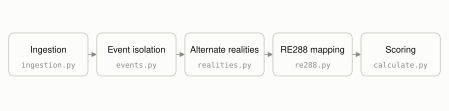
\includegraphics[width=0.95\textwidth]{../outputs/figures/pipeline_diagram.svg}
    \caption{CRV pipeline from ingestion to scoring outputs.}
    \label{fig:pipeline}
\end{figure}

\section{Preliminary Results}
Executable experiment outputs are written to \texttt{outputs/}. In this environment, the pipeline falls back to synthetic challenge events when full Statcast retrieval is unavailable. The produced artifacts include:
\begin{itemize}
    \item \texttt{challenge\_events\_scored.csv}
    \item \texttt{player\_leaderboard.csv}
    \item \texttt{challenger\_summary.csv}
    \item SVG figures for leaderboard and challenger totals.
\end{itemize}

\begin{figure}[h]
    \centering
    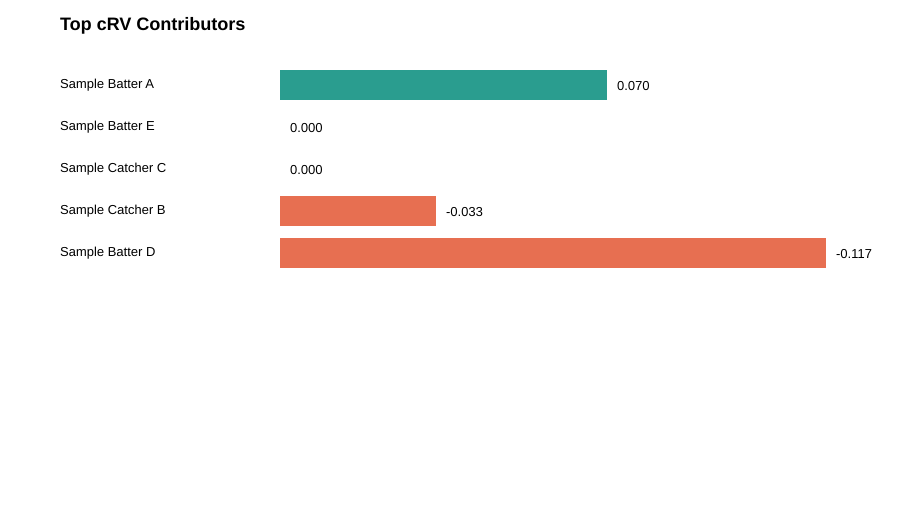
\includegraphics[width=0.95\textwidth]{../outputs/figures/leaderboard_top10.svg}
    \caption{Top contributors by cumulative $cRV$ (current run output).}
\end{figure}

\section{Discussion}
The current implementation establishes a reproducible baseline and audit trail for $cRV$ construction. Next empirical milestones are full 2026 data pull, calibrated RE288 from historical play-by-play, sensitivity testing over $EV_c$, and robustness checks by leverage context.

\section{Conclusion}
$cRV$ offers a practical framework for measuring challenge strategy in the ABS era and is ready for expansion into full-season evaluation and player-level stability analysis.

\bibliographystyle{plain}
\bibliography{references}

\end{document}
